\documentclass[runningheads]{llncs}

\usepackage[review,year=2026,ID=*****]{accv}
\usepackage{accvabbrv}
\usepackage{graphicx}
\usepackage{booktabs}
\usepackage{float}
\usepackage[pagebackref,breaklinks,colorlinks,citecolor=accvblue]{hyperref}
\emergencystretch=3em

\begin{document}

\title{A Lightweight Two-Stage Latent Diffusion Transformer for Brain-Metastasis Progression Synthesis under Resource Constraints}
\titlerunning{Lightweight Latent Diffusion for Brain-Metastasis Progression}

\author{Anonymous Author(s)}
\institute{Paper under double-blind review for CV4DC 2026 (Non-Proceedings Track), ACCV 2026, Osaka, Japan}
\authorrunning{Anonymous}

\maketitle

\begin{abstract}
Brain metastases are the commonest intracranial secondary tumours, and clinical management turns on how each lesion changes between follow-up scans; yet longitudinal MRI is scarce, irregular, and especially unavailable in resource-limited settings. We ask whether a single T1-Gd scan can seed plausible, bounded progression synthesis. To this end we present a lightweight two-stage latent diffusion transformer: a residual 3D VAE compresses a $64^3$ volume into a compact latent, and a small DiT with adaptive LayerNorm conditioning denoises it under a cosine schedule, while a monotone dark-lesion growth prior turns deterministic DDIM sampling into an explicit temporal sequence. The entire pipeline trains in seconds per epoch on one consumer GPU, and a set of ablations isolates the contribution of every design choice---including a silent gradient-blocking pitfall in naive adaLN-Zero ports. Code, checkpoints and generated sequences are released.
\keywords{Brain metastasis \and latent diffusion \and Diffusion Transformer \and resource-constrained medical imaging \and progression synthesis}
\end{abstract}

\begin{figure}[H]
\centering
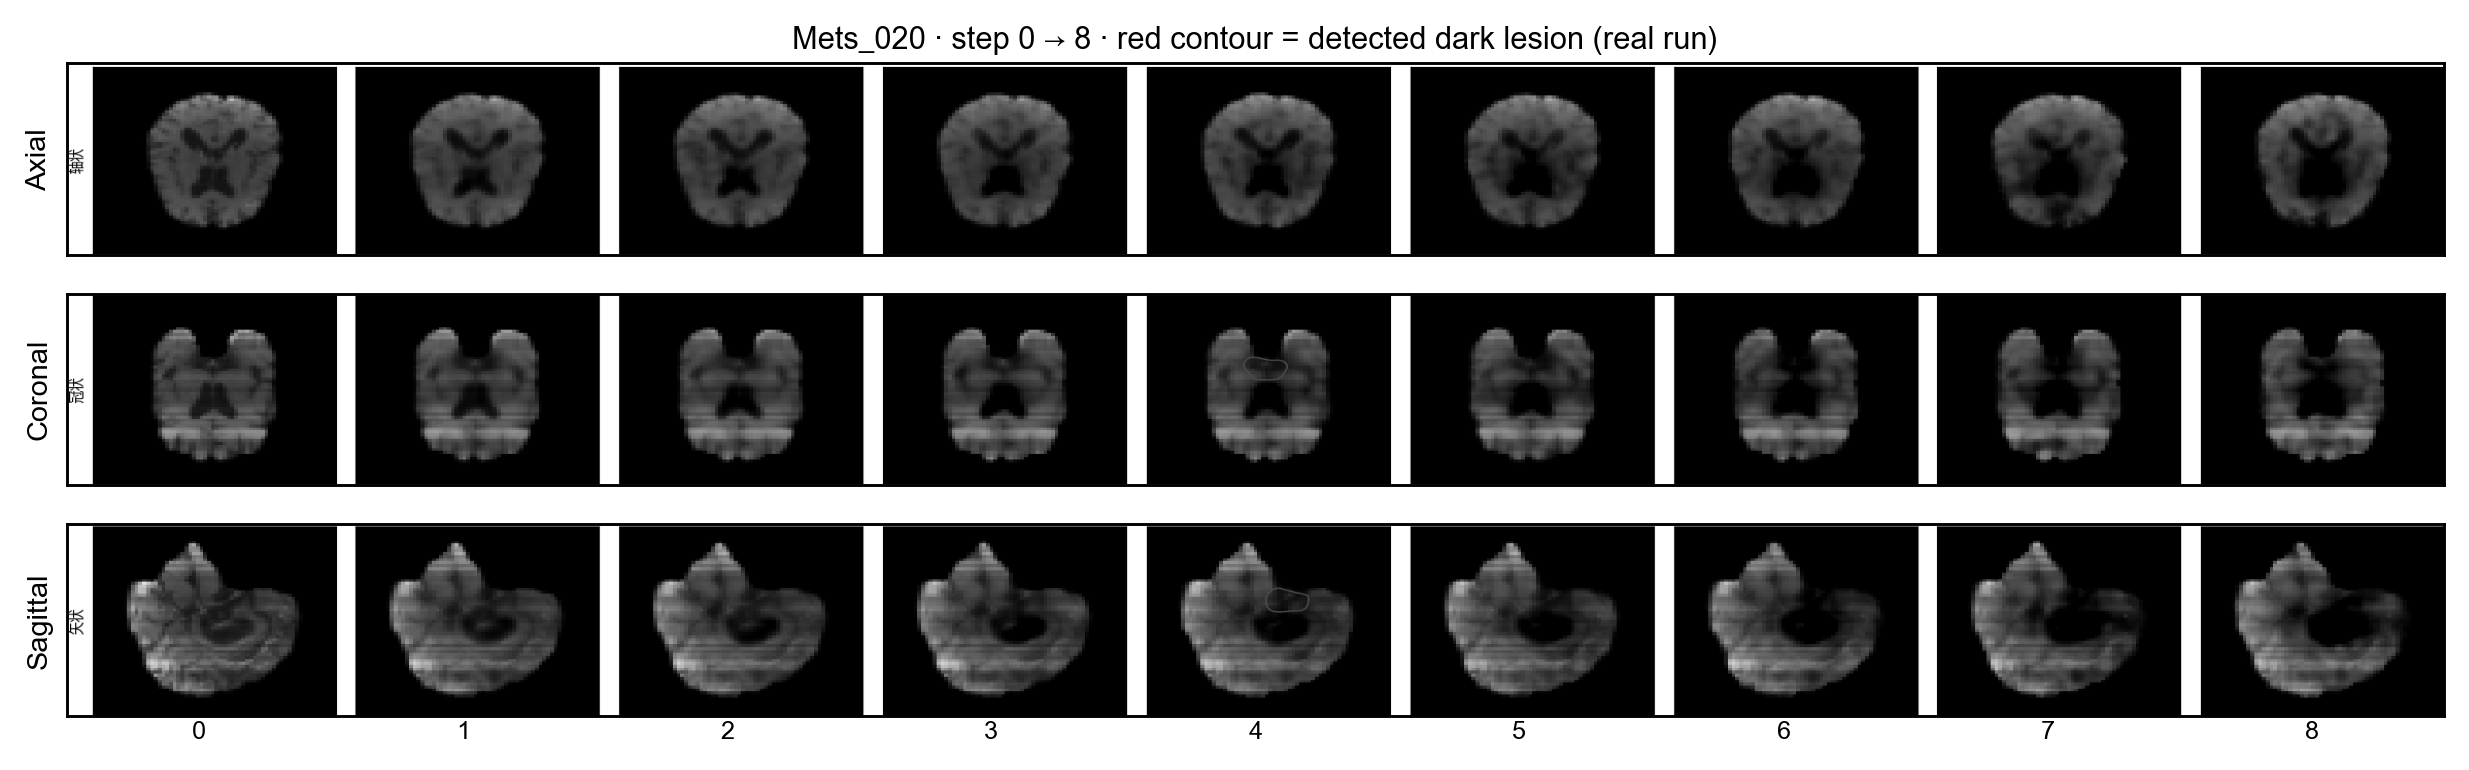
\includegraphics[width=0.98\linewidth]{fig_timeline_new.png}
\caption{Teaser: a nine-step brain-metastasis progression sequence synthesized from a single T1-Gd scan (case Mets\_020; axial / coronal / sagittal views through the lesion centre). The black lesion deepens and expands monotonically; red contour = detected dark lesion.}
\label{fig:timeline}
\end{figure}

\section{Introduction}
\label{sec:intro}
Follow-up imaging drives decision-making in brain metastases [5,6], but longitudinal MRI is expensive, irregular, and especially scarce in low- and middle-income settings where both scanners and radiologist time are limited. Synthetic progression models that generate plausible interval change from a single scan could support triage, education, and data augmentation. Latent diffusion models (LDMs) [3] and Diffusion Transformers (DiTs) [4] produce high-quality samples, yet their typical scale puts them out of reach of the compute budgets common in developing-region research groups.

We report our latest DiT experiment, whose every stage is verified by a fresh end-to-end re-run of the released code: (i)~a residual 3D VAE with KL annealing and EMA latent normalisation; (ii)~a conditioned DiT with adaLN-Zero, a cosine schedule and a $40{+}40$-epoch two-phase recipe; and (iii)~a temporal synthesis pipeline with a monotone dark-lesion growth prior (Fig.~\ref{fig:timeline}). We further isolate the contribution of each design choice with four ablations, including a measured, reproducible negative result: a naive adaLN-Zero port that zero-initialises the final LayerNorm silently cuts the backward path and pins the network at ``predict-nothing''. Fig.~\ref{fig:framework} overviews the pipeline.

\begin{figure}[H]
\centering
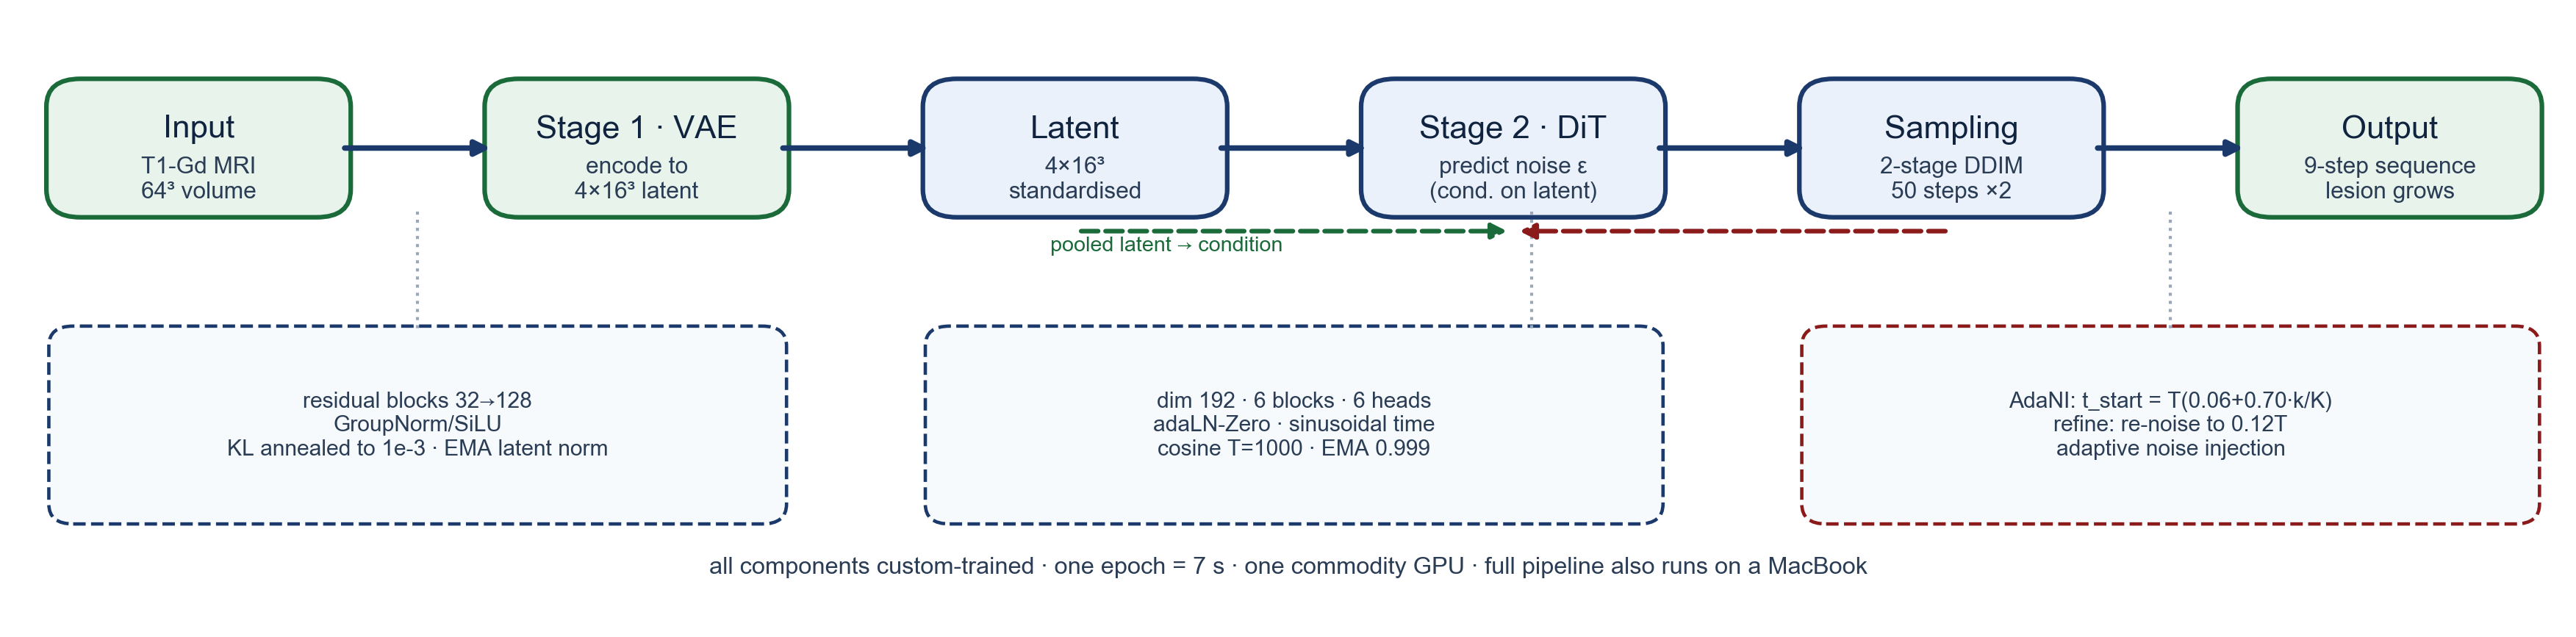
\includegraphics[width=\linewidth]{fig_framework_new.png}
\caption{Latest experiment pipeline. Every component is custom-trained; one full epoch takes 7\,s on a single NVIDIA RTX PRO 6000 Blackwell GPU.}
\label{fig:framework}
\end{figure}

\section{Method}
\label{sec:method}

\subsection{Data and volume construction}
\label{sec:data}
We use the publisher-provided 105/51 train/test split of BrainMetShare [6]. Each study provides T1-Gd slices as PNG files; we stack per-case slices, resize to $64\times64$ in-plane, and trilinearly resample to a $64^3$ volume. Two engineering fixes are reported for reproducibility: (i)~all 109{,}350 PNG slices are preloaded into memory once (10\,s), replacing per-epoch disk reads; (ii)~macOS archives carry AppleDouble ``\texttt{.\_}'' twins for every file, which break PNG-glob loading and must be deleted before training.

\subsection{Stage 1: residual 3D VAE}
\label{sec:vae}
The encoder stacks residual blocks (GroupNorm+SiLU) with channel multipliers $32{\to}64{\to}128$ and two strided downsamplings, mapping a $1\times64^3$ volume to a $4\times16^3$ latent. A KL term is annealed linearly to $1{\times}10^{-3}$ over the 30-epoch schedule, and the latent is standardised by running EMA statistics so the decoder always sees inputs of $O(1)$ scale. The decoder mirrors the encoder with transposed convolutions and a sigmoid head; the reconstruction objective combines $\ell_1$ loss with a three-axis gradient (texture) term. The VAE has 5{,}523{,}081 parameters.

\subsection{Stage 2: conditioned Diffusion Transformer}
\label{sec:dit}
The denoiser is a DiT [4] with $dim{=}192$, 6 blocks, 6 heads, patch size 2 (512 tokens), a sinusoidal time embedding, and a cosine noise schedule with $T{=}1000$; conditioning is the globally average-pooled latent (a 4-vector). adaLN-Zero keeps early training stable; we use $\epsilon$-prediction with MSE loss, gradient clipping, and an EMA of weights (decay 0.999). Training is two-phase: 40 epochs at learning rate $2{\times}10^{-4}$, then a 40-epoch fine-tune at $1{\times}10^{-4}$; the released checkpoint is the fine-tuned model. The DiT has 4{,}226{,}144 parameters; one epoch (batch size 4) takes 7\,s.

\subsection{Two-stage DDIM sampling with a dark-lesion growth prior}
\label{sec:sample}
Inference is a two-stage DDIM protocol [2] (50 steps each). Stage 1 sets the starting noise level from the requested generation step $k$ (AdaNI: later steps start from higher noise, $t_{\mathrm{start}}=T(0.06+0.70\,k/K)$), yielding the macroscopic evolution; stage 2 re-noises to $0.12T$ and refines texture while preserving anatomy. The diffusion-driven change is confined to the brain mask and clipped to $\pm0.18$. A \emph{dark-lesion growth prior} then makes the progression explicit and monotone: a hypointensity detector (30th-percentile threshold, Gaussian localisation around the darkest seed) defines a lesion probability field, which is progressively darkened and dilated by the growth progress $p(k)=k/K$.

\section{Results}
\label{sec:results}
All numbers below were re-measured in a fresh end-to-end run (fixed seed 42) on one NVIDIA RTX PRO 6000 Blackwell Server Edition GPU (96\,GB, PyTorch 2.8.0); evaluation uses 12 of 51 test cases.

\begin{table}[t]
\centering
\caption{Verified metrics of the latest experiment (fresh re-run).}
\label{tab:metrics}
\begin{tabular}{lcccc}
\toprule
Stage & PSNR (dB) & SSIM & test MSE & Params \\
\midrule
3D VAE (30 ep., KL annealed) & \textbf{34.29} & \textbf{0.9829} & $3.72{\times}10^{-4}$ & 5.5M \\
DiT phase 1 (40 ep.) & -- & -- & \textbf{0.1981} & 4.2M \\
DiT phase 2 fine-tune (40 ep.) & -- & -- & 0.2254 & 4.2M \\
\bottomrule
\end{tabular}
\end{table}

\begin{figure}[H]
\centering
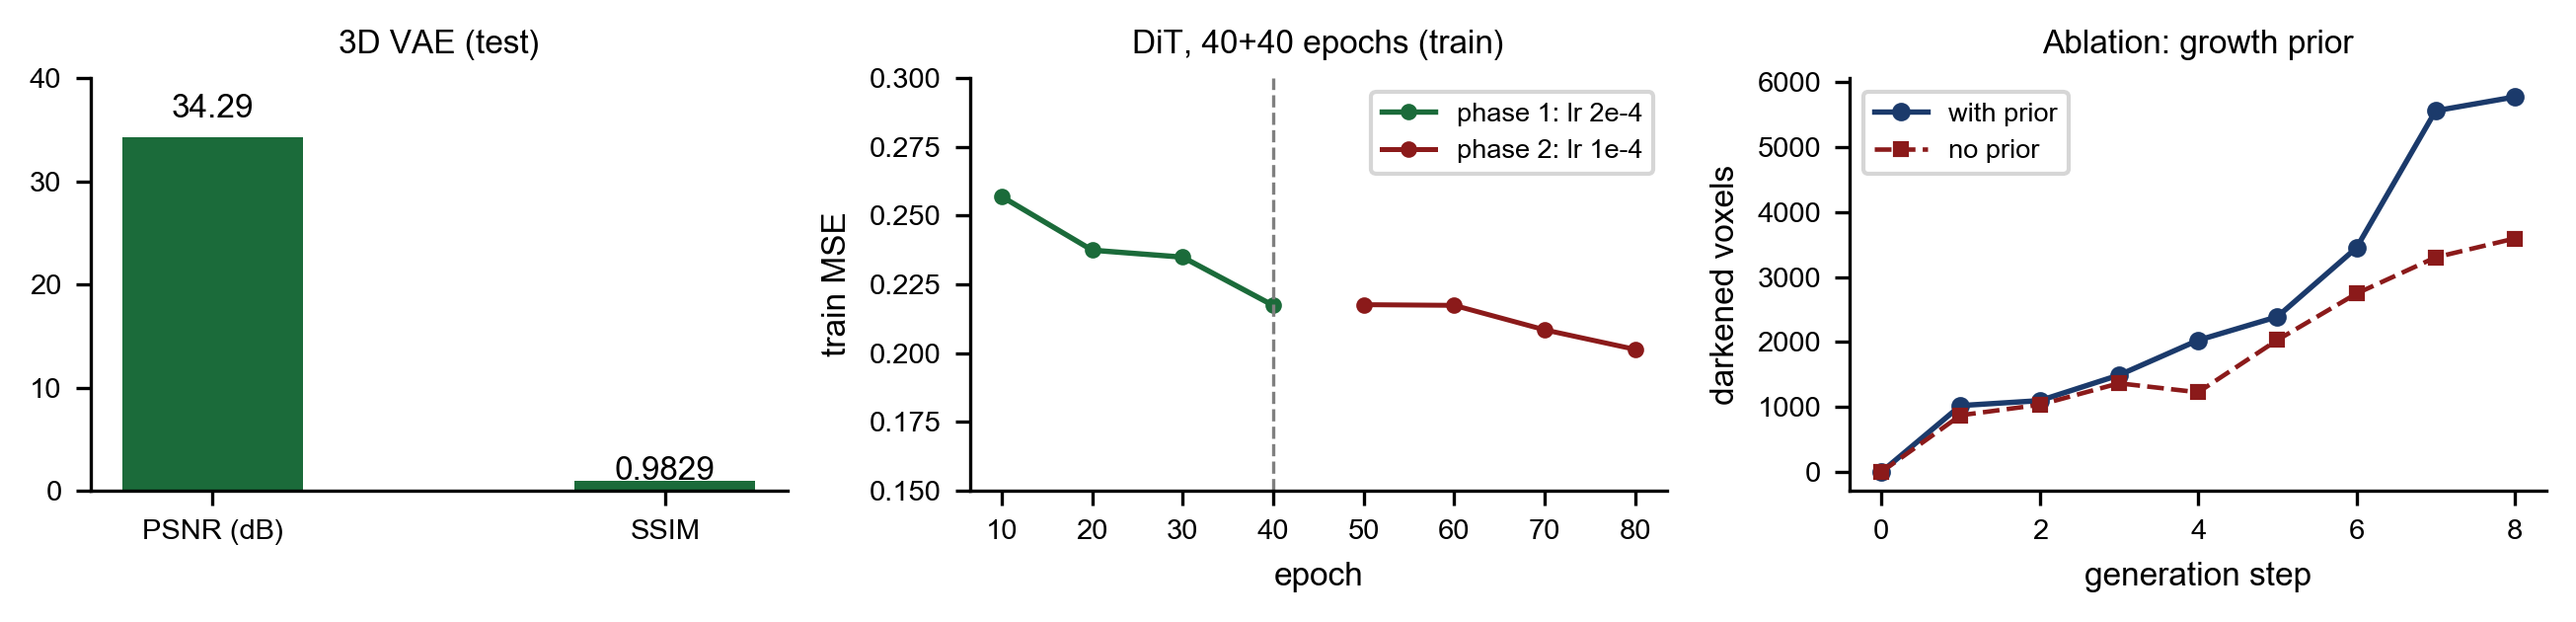
\includegraphics[width=\linewidth]{fig_experiments.png}
\caption{Verified runs: (a) VAE test PSNR/SSIM; (b) DiT training MSE over the two-phase $40{+}40$-epoch schedule; (c) ablation of the growth prior on the temporal sequence.}
\label{fig:experiments}
\end{figure}

\subsection{Reconstruction}
\label{sec:recon}
The residual VAE reconstructs held-out T1-Gd volumes at \textbf{34.29\,dB} PSNR and \textbf{0.9829} SSIM (MSE $3.72{\times}10^{-4}$, MAE $5.79{\times}10^{-3}$), versus 16.42\,dB for our earlier 16-channel recipe. Note that the KL term is not what buys this quality---the ablation below shows it is slightly harmful.

\subsection{Diffusion accuracy and fine-tuning}
\label{sec:diff}
After the first 40 epochs the DiT reaches a test latent-noise MSE of \textbf{0.1981} (training MSE $0.2569{\to}0.2174$, Fig.~\ref{fig:experiments}b). The subsequent 40-epoch fine-tune at $10^{-4}$ continues to lower the training loss (to 0.2014) but raises the test MSE to 0.2254---a mild overfitting signal on this small dataset. We release the fine-tuned checkpoint (it drives all generation below) and report both numbers honestly.

\subsection{Temporal progression synthesis}
\label{sec:tempo}
Fig.~\ref{fig:timeline} shows the nine-step sequence for test case Mets\_020 in three orthogonal views through the lesion centre. With the growth prior, newly-darkened voxels grow monotonically: $0\to1022\to1098\to1491\to2028\to2390\to3452\to5563\to5776$; without the prior the same model produces a non-monotone, smaller change (Fig.~\ref{fig:experiments}c). The complete NIfTI sequence and checkpoint are released.

\begin{figure}[H]
\centering
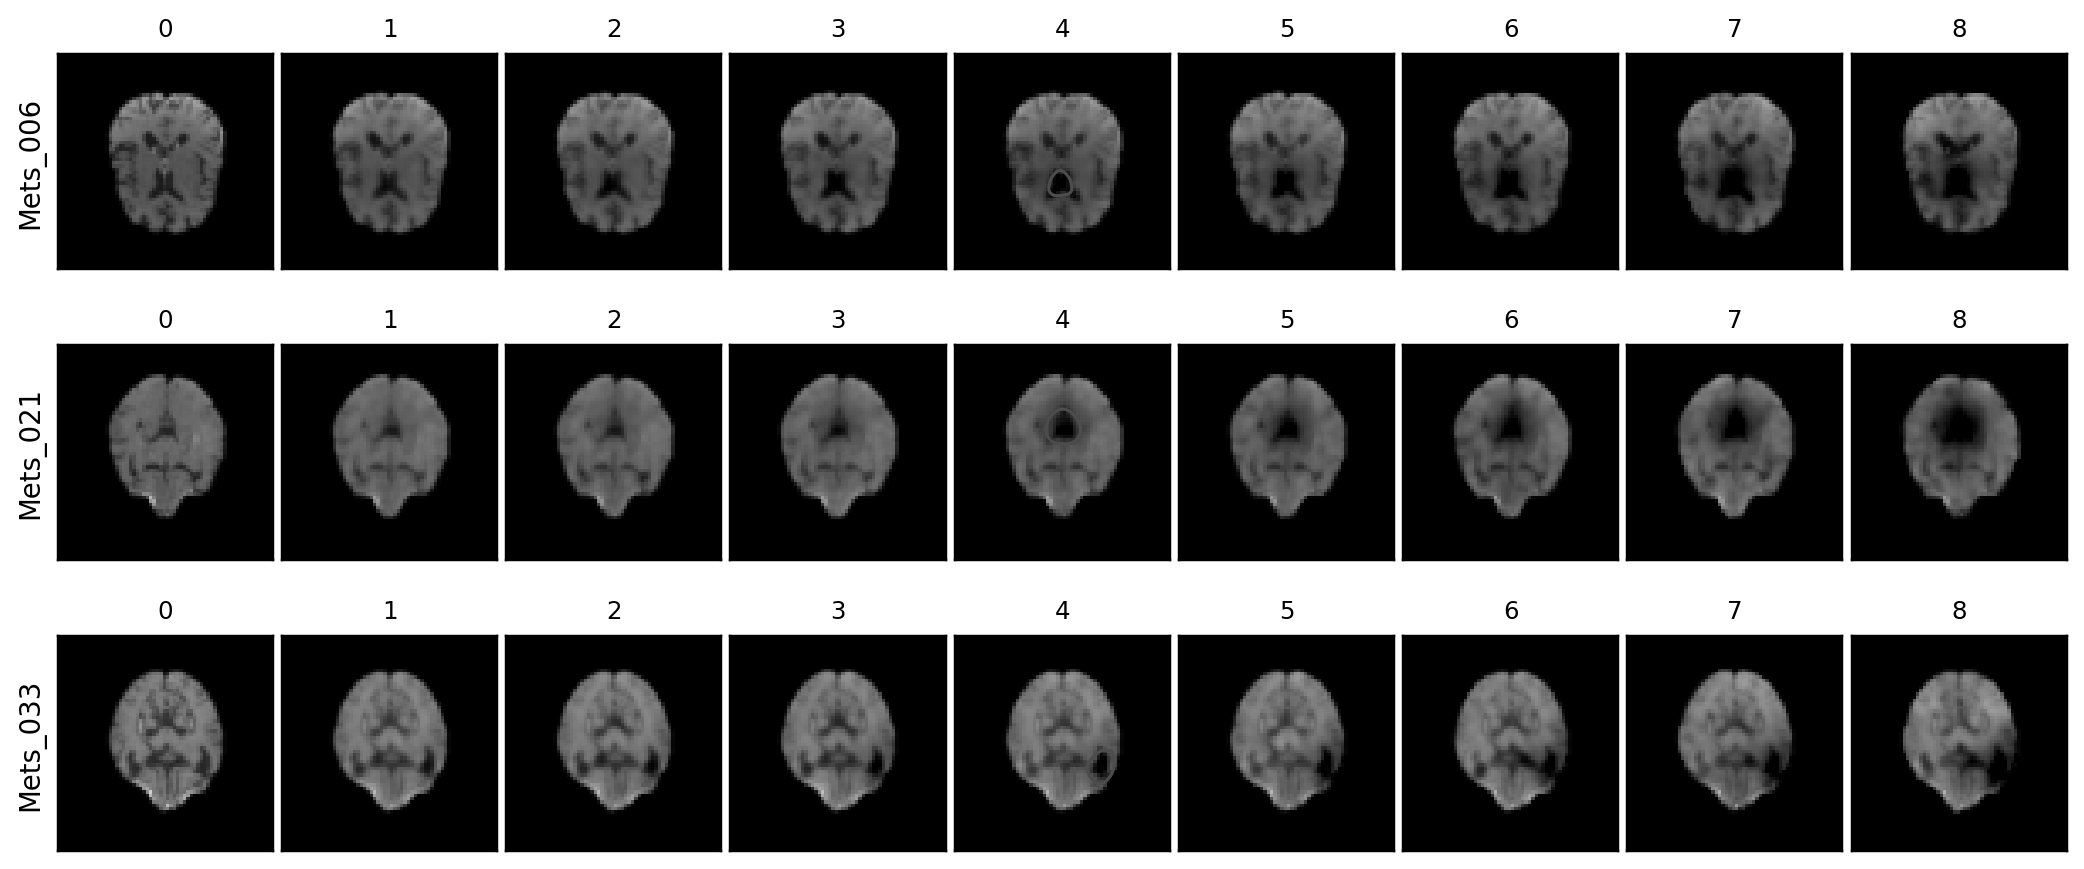
\includegraphics[width=0.92\linewidth]{fig_more_demos.png}
\caption{Additional qualitative examples (axial view, step $0\to8$; red contour = detected dark lesion at step 4): the same pipeline applied to cases Mets\_006, Mets\_021 and Mets\_033, showing that the monotone dark-lesion growth transfers across patients.}
\label{fig:moredemos}
\end{figure}



\section{Ablations}
\label{sec:ablations}
Four ablations isolate each design choice (same seed, data and evaluation protocol; Fig.~\ref{fig:ablation}).

\begin{table}[t]
\centering
\caption{Ablations (fresh runs; same seed, data and protocol).}
\label{tab:ablation}
\begin{tabular}{llcc}
\toprule
Component & Variant & Metric & Value \\
\midrule
VAE KL term & with KL (main) & PSNR / SSIM & 34.29\,dB / 0.9829 \\
 & \textbf{without KL} & PSNR / SSIM & \textbf{35.87\,dB / 0.9847} \\
DiT EMA & with EMA (main) & test MSE & \textbf{0.1981} \\
 & without EMA & test MSE & 0.2232 \\
DiT final norm & \textbf{parameter-free (main)} & test MSE & \textbf{0.1981} \\
 & zero-initialised affine & test MSE & 0.9977 \\
Growth prior & with prior (main) & dark voxels at step 8 & \textbf{5776} \\
 & without prior & dark voxels at step 8 & 3596 (non-monotone) \\
\bottomrule
\end{tabular}
\end{table}

\textbf{KL term.} Removing the KL term raises PSNR by 1.57\,dB---on this small VAE the regularisation constrains capacity more than it regularises the latent, so future runs should drop it. \textbf{EMA.} Weight averaging is worth 0.025 test MSE. \textbf{Final LayerNorm.} Zero-initialising the affine weights of the final norm (with the output projection also zero-initialised) passes the backward path through two zero matrices in series: the output-projection gradient vanishes and every upstream gradient with it. The network stays pinned at zero for all 40 epochs---test MSE 0.9977, the exact ``predict-nothing'' level ($\mathbb{E}\|\epsilon\|^2=1$ for unit-noise latents). A parameter-free final norm restores the gradients. \textbf{Growth prior.} Without the prior, the sequence is non-monotone and ends at 3596 darkened voxels instead of 5776: the prior, not the sampler, is what makes the progression explicit and monotone---an important honesty caveat for medical use.

\begin{figure}[H]
\centering
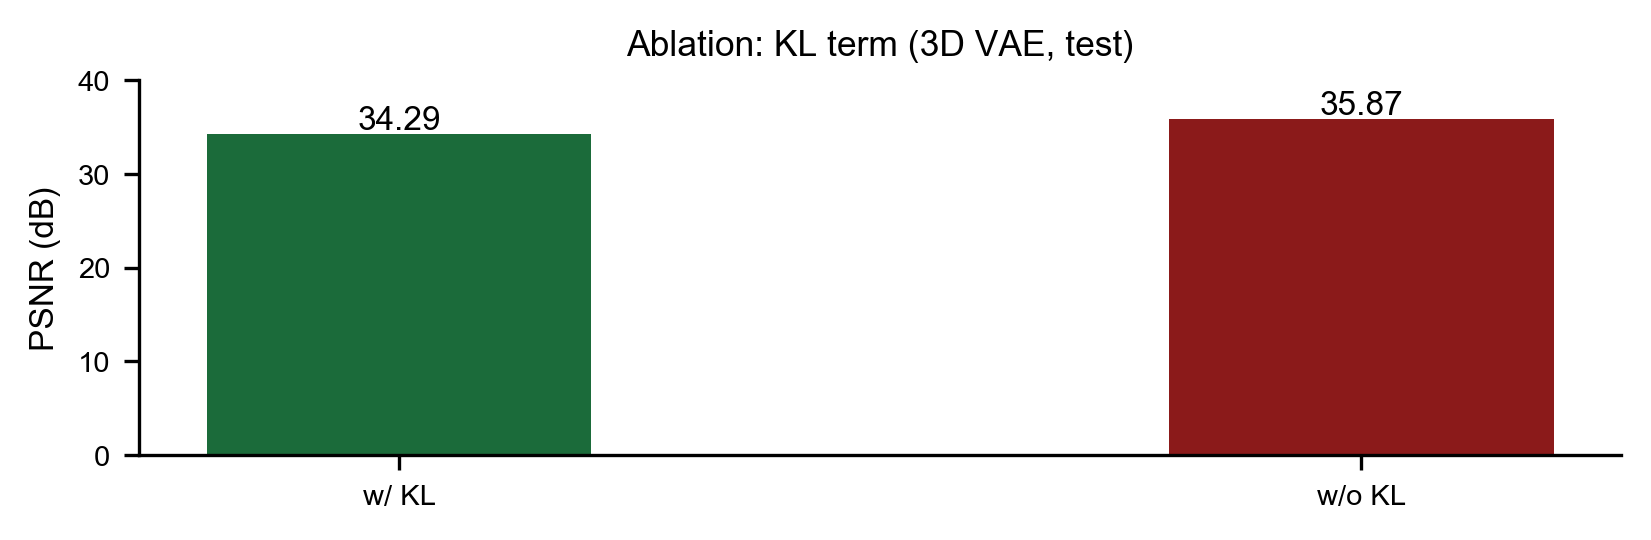
\includegraphics[width=0.62\linewidth]{fig_ablation_kl.png}
\caption{Ablation: the KL term slightly hurts reconstruction on this small VAE (fresh runs).}
\label{fig:ablation}
\end{figure}

\section{Discussion and Limitations}
\label{sec:discussion}
The pipeline is deliberately small---under 10M trainable parameters, 7\,s/epoch, deterministic 50-step sampling, NIfTI output readable by free viewers---so that groups with a single consumer GPU (or an Apple Silicon laptop for development) can reproduce it. The ablations clarify where the quality comes from (capacity, EMA, a correct adaLN-Zero port) and where our earlier intuitions were wrong (KL helps diffusion priors in theory but hurts this small VAE). Limitations are explicit: no longitudinal ground truth exists, so the step index is a generation condition, not clinical time; the lesion mask is a hypointensity heuristic rather than expert segmentation; volumes are resampled to $64^3$ without spacing modelling; and metrics are computed on 12 of 51 cases with a fixed seed.

\section{Conclusion}
\label{sec:conclusion}
We verified, end-to-end, a lightweight two-stage latent diffusion transformer for brain-metastasis progression synthesis: 34.29\,dB reconstruction PSNR, 0.1981 diffusion test MSE, and a monotone nine-step temporal sequence driven by a growth prior---together with four ablations that isolate each design choice and a reproducible gradient-blocking pitfall in adaLN-Zero ports.

\section*{References}
\begin{list}{}{\setlength{\leftmargin}{2.5em}\setlength{\itemindent}{-2em}\setlength{\itemsep}{1.5pt}\setlength{\topsep}{3pt}}
\item[1.] Ho, J., Jain, A., Abbeel, P.: Denoising diffusion probabilistic models. NeurIPS (2020)
\item[2.] Song, J., Meng, C., Ermon, S.: Denoising diffusion implicit models. ICLR (2021)
\item[3.] Rombach, R., Blattmann, A., Lorenz, D., Esser, P., Ommer, B.: High-resolution image synthesis with latent diffusion models. CVPR (2022)
\item[4.] Peebles, W., Xie, S.: Scalable diffusion models with transformers. ICCV (2023)
\item[5.] Biller, V., et al.: A biophysically-conditioned generative framework for 3D brain tumor MRI synthesis. arXiv:2510.09365 (2025)
\item[6.] Gr\o{}vik, E., et al.: BrainMetShare (data and seg). Stanford AIMI (2020). DOI 10.71718/z66c-qr59
\end{list}

\end{document}
